\documentclass[10pt]{report}
\usepackage{/Users/bradenhoagland/latex/math}

\lhead{Braden Hoagland}
\chead{Category Theory}
\rhead{}

\newcommand{\cat}[1]{\mathsf{#1}}
\DeclareMathOperator{\hh}{Hom}
\DeclareMathOperator{\op}{op}
\DeclareMathOperator{\ob}{ob}

\begin{document}
\tableofcontents

%%%%%%%%%%%%%%%%%%%%
% Categories
%%%%%%%%%%%%%%%%%%%%

\section{Categories}

\begin{defn}
	A \textbf{category} $\cat{C}$ is a class of \textbf{objects} $\ob(\cat{C})$ along with sets of \textbf{morphisms} between those objects. The set of morphisms $A$ to $B$ is denoted $\hh_{\cat{C}}(A,B)$ or $\cat{C}(A,B)$. There must be a law of composition of morphisms
	\[
		(f, g) \mapsto gf.
	\] Finally, the objects and morphisms satisfy:
	\begin{enumerate}
		\item If $A \neq C$ or $B \neq D$, then $\hh_{\cat{C}}(A,B)$ and $\hh_{\cat{C}}(C,D)$ are disjoint sets.
		\item Morphism composition is associative.
		\item Each object has an identity morphism.
	\end{enumerate}
\end{defn}

We will drop the subscript $\cat{C}$ in $\hh_{\cat{C}}$ if the category is clear.

\begin{defn}
	A category $\cat{S}$ is a \textbf{subcategory} of $\cat{C}$ if
	\begin{enumerate}
		\item $\ob(\cat{S})$ is a subclass of $\ob(\cat{C})$; and
		\item for all $A, B \in \ob(\cat{S})$, $\hh_{\cat{S}}(A,B)$ is a subclass of $\hh_{\cat{C}}(A,B)$.
	\end{enumerate}
	A \textbf{full} subcategory maintains all morphisms from $\cat{C}$ among the objects that it maintains, i.e. for $A, B \in \ob(\cat{S})$, $\hh_{\cat{S}}(A,B) = \hh_{\cat{C}}(A,B)$.
\end{defn}

\begin{note}
The image of a category need not be a subcategory.
\end{note}

\begin{prop}
The identity morphism of an object is unique.
\end{prop}
\begin{proof}
	Suppose $1_{A}$ and $1_{A}'$ are both identity morphisms of $A$. Then $1_{A}=1_{A}1_{A}'=1_{A}'$.
\end{proof}

\begin{defn}
An \textbf{endomorphism} of $A$ is a morphism from $A$ to itself.
\end{defn}

\begin{defn}
	An \textbf{isomorphism} $f:A\to B$ is an invertible morphism, i.e. there exists a morphism $g:B\to A$ such that $gf=1_{A}$ and $fg=1_{B}$.
\end{defn}

\begin{prop}
Inverses of morphisms are unique.
\end{prop}
\begin{proof}
Suppose $f:A \to B$ is a morphism and $g,g': B \to A$ are both inverses of it. Then by associativity of morphism composition, $g=g1_{B}=g(fg')=(gf)g'=1_{A}g'=g'.$
\end{proof}

\begin{defn}[]
A \textbf{groupoid} is a category whose morphisms are all isomorphisms. Every category contains a subcategory called the \textbf{maximal groupoid}, which is all of the objects along with only the morphisms that are isomorphisms.
\end{defn}

\begin{ex}[]
	We can define a \textbf{group} as a groupoid that has only one object. The group elements are the morphisms. The properties of a group follow from the properties of categories and the fact that our morphisms are all isomorphisms.
\end{ex}

{\color{red}Put picture of group and groupoid as category.}

Now for some examples to make this \textit{somewhat} less abstract.

\begin{enumerate}
	\item \textbf{Set}: the category of all sets. The category of all finite sets is a subcategory of this.
		\begin{itemize}
			\item $\hh(A,B)$ is the set of all functions from $A$ to $B$.
			\item Morphism composition is the usual composition of functions.
			\item The identity morphism sends $a \in A$ to itself.
		\end{itemize}
	\item \textbf{Grp}: the category of all groups. \textbf{Ab}, the category of all abelian groups, is a subcategory of this. Morphisms are group homomorphisms, and isomorphisms are, well, group isomorphisms.
	\item \textbf{Ring}: the category of all nonzero rings with $1$. The morphisms are ring homomorphisms that send 1 to 1.
	\item \textbf{R-mod}: the category of all left $R$-modules. The morphisms are $R$-module homomorphisms.
	\item \textbf{Top}: the category of all topological spaces. The morphisms are continuous maps between spaces, and the isomorphisms are homeomorphisms.
\end{enumerate}

\begin{defn}
A \textbf{discrete category} is a category in which all the morphisms are identities, i.e. every object is isolated.
\end{defn}

\begin{defn}
	Given a category $\cat{C}$, its \textbf{opposite} or \textbf{dual} category $\cat{C}^{\text{op}}$ is the category gotten by reversing the morphisms of $\cat{C}$. Formally, $\ob(\cat{C}^{\op}) = \ob(\cat{C})$, but
	\[
		\hh_{\cat{C}^{\text{op}}}(A,B) = \hh_{\cat{C}}(B,A).
	\] 
\end{defn}

Note that the identities in a category and its dual are the same. Compositions, on the other hand, are reversed.

\begin{figure}[H]
	\centering
\begin{tikzcd}
\bullet \arrow[r, "f"] \arrow[rd, "gf"'] & \bullet \arrow[d, "g"] &  & \bullet & \bullet \arrow[l, "f'"']                    \\
                                         & \bullet                &  &         & \bullet \arrow[lu, "f'g'"] \arrow[u, "g'"']
\end{tikzcd}
	\caption{A category and its dual. Since every object must have an identity morphism, I usually won't include them in a diagram unless necessary.}
\end{figure}

\begin{defn}
Given categories $\cat{C}$ and $\cat{D}$, we can define their \textbf{product category} $\cat{C} \times \cat{D}$ as having the objects
\[
	\ob(\cat{C} \times \cat{D}) = \ob(\cat{C}) \times \ob(\cat{D})
\] and the morphisms
\[
	\hh_{\cat{C} \times \cat{D}}( (A,B), (A',B') ) = \hh_{\cat{C}}(A,A') \times \hh_{\cat{D}}(B,B').
\] 
\end{defn}
It is straightforward to define the identity morphisms and the composition of morphisms in product categories in a piecewise fashion, building off the identities and composition laws of $\cat{C}$ and $\cat{D}$.

%%%%%%%%%%%%%%%%%%%%
% Universal Properties
%%%%%%%%%%%%%%%%%%%%

\section{Universal Properties}

\begin{defn}[]
	An object $A$ is \textbf{initial} if there is a unique morphism $A \to B$ for all objects $B$. An object $C$ is \textbf{final} if there is a unique morhpism $B \to C$ for all objects $C$. An object that is either initial or fianl is called \textbf{universal}, and it's a \textbf{zero object} if it's both.
\end{defn}

\begin{ex}[]
In \textbf{Grp}, the trivial group $\left\{ 1 \right\}$ is a zero object.
\end{ex}

\begin{prop}
	All initial objects are isomorphic. All final objects are isomorphic.
\end{prop}
\begin{proof}
	If $A,A'$ are both initial, there are unique morphisms $f:A\to A'$ and $g:A'\to A$. Then $gf$ is a morphism $A\to A$. Since $A$ is universal, it has only one endomorphism, namely the identity map. Thus $gf=1_{A}$. Similarly, $fg=1_{A'}$. Thus $A \cong A'$. The proof is similar for final objects.
\end{proof}

\begin{ex}[]
If we have a morphism $f:X\to Y$, we can define an equivalence relation
\[
	a \sim b \iff f(a) = f(b).
\] Then if $\pi$ is the canonical projection map, the following diagram commutes.
\begin{figure}[H]
	\centering
\begin{tikzcd}
X/\sim \arrow[rr, "\exists!\;g", dashed]       &  & Y \\
                                       &  &   \\
X \arrow[uu, "\pi"] \arrow[rruu, "f"'] &  &  
\end{tikzcd}
\end{figure}

Consider the category with objects the morphisms $X\to Y$ that respect $\sim$ and morphisms given by push-forwards. In this category, $\pi$ is initial (and thus universal). Colloquially, we say that $X/\sim$ has this universal property, although it's really $\pi$ that has the property. But $\pi$ is the only map $X \to  X/\sim$ that makes sense, though, so we can say either and it's obvious what we mean.

{\color{red}Is $\im f \cong X/\sim$ for all categories? Seems like it should depend on what the canonical projection is in the particular category...}
\end{ex}

%%%%%%%%%%%%%%%%%%%%
% Functors
%%%%%%%%%%%%%%%%%%%%

\section{Functors}

Functors map categories to categories by associating objects with objects and morphisms with morphisms in ways that respect morphism composition and identities.

\begin{figure}[H]
	\centering
	\begin{tikzcd}
                                                   & B \arrow[dd, "g"] \arrow[rrr, dashed] &  &                                           & \mathcal{F}B \arrow[dd, "\mathcal{F}(g)"] \\
A \arrow[ru, "f"] \arrow[rrr, dashed, shift right] &                                       &  & \mathcal{F}A \arrow[ru, "\mathcal{F}(f)"] &                                           \\
                                                   & C \arrow[lu, "h"] \arrow[rrr, dashed] &  &                                           & \mathcal{F}C \arrow[lu, "\mathcal{F}(h)"]
\end{tikzcd}
\caption{A functor $\mathcal{F}$ between two categories.}
\end{figure}

\begin{defn}
	A \textbf{functor} $\mathcal{F}:\cat{C}\to \cat{D}$ satisfies:
\begin{enumerate}
	\item For every object $A$ in $\cat{C}$, $\mathcal{F}A$ is an object in $\cat{D}$.
	\item For every $f \in \hh_{\cat{C}}(A,B)$, $\mathcal{F}(f)$ is a morphism in $\hh_{\cat{D}}(\mathcal{F}A, \mathcal{F}B)$ such that
		\begin{enumerate}
			\item $\mathcal{F}(gf) = \mathcal{F}(g) \mathcal{F}(f)$, and
			\item $\mathcal{F}(1_{A}) = 1_{\mathcal{F}A}$.
		\end{enumerate}
\end{enumerate}
	Sometimes we call a functor a \textbf{covariant functor} to differentiate it from another type of functor, which we define in a bit.
\end{defn}

\begin{ex}[Category Inception]
The category \textbf{CAT} has objects that are themselves categories, and its morphisms are functors.
\end{ex}

\begin{defn}
	Given a functor $f \in \hh_{\cat{C}}(A,B)$, $A$ is the \textbf{domain} and $B$ is the \textbf{codomain} of $f$.
\end{defn}

There are tons of examples of functors, so here are some that aren't too complicated.
\begin{enumerate}
	\item The \textbf{identity functor} $\mathcal{I}_{\cat{C}}$ maps $\cat{C}$ to $\cat{C}$ by sending objects and morphims to themselves.
	\item If $\cat{C}$ is a subcategory of $\cat{D}$, then the \textbf{inclusion functor} maps $C$ to $D$ by sending objects and morphisms to themselves, except now as members of $\cat{D}$ instead of $\cat{C}$.
	\item \textbf{Forgetful functors} take a category and strip its objects of some kind of complexity, i.e. a functor from \textbf{Grp} to \textbf{Set}. A forgetful functor doesn't have to just map objects to plain sets, though. We could also map \textbf{Ab} to \textbf{Grp}, forgetting the abelian nature of the groups in our category.
\end{enumerate}

{\color{red}More examples.}

In order to ``respect" morphisms, we might either keep the morphisms all in the same direction or flip them. If we decide to flip them all, we get a different type of functor.

\begin{prop}
Functors preserve isomorphisms.
\end{prop}
\begin{proof}
	Suppose $\mathcal{F}:\cat{A}\to \cat{B}$ is a functor, and suppose $A \cong A'$ are isomorphic objects in $\cat{A}$. Since $A$ and $A'$ are isomorphic, there are inverses $f:A\to A'$ and $g:A'\to A$. By definition, $\mathcal{F}(f)$ and $\mathcal{F}(g)$ can be composed and
	\[
		\mathcal{F}(f)\mathcal{F}(g) = \mathcal{F}(fg) = \mathcal{F}(1_{A'}) = 1_{\mathcal{F}A'}.
	\] Similarly, $\mathcal{F}(g)\mathcal{F}(f)=1_{\mathcal{F}A}$, so $\mathcal{F}A \cong \mathcal{F}A'$.
\end{proof}

\begin{defn}
	A \textbf{contravariant functor} from $\cat{C}$ to $\cat{D}$ is a functor from $\cat{C}^{\op}$ to $\cat{D}$.
\end{defn}

\begin{defn}
A functor $\mathcal{F}:\cat{C}\to \cat{D}$ is \textbf{faithful} if for all objects $A,B$ of $\cat{C}$, the map
\begin{align*}
	\hh_{\cat{C}}(A,B) &\to \hh_{\cat{D}}(\mathcal{F}A, \mathcal{F}B) \\
	f &\mapsto \mathcal{F}(f)
\end{align*} is one-to-one. $\mathcal{F}$ is \textbf{full} if this map is onto.
\end{defn}

Note that the fixed $A$ and $B$ above are important. The injective/surjective conditions don't apply to arbitrary morphisms in $\cat{C}$ since they might connect different objects.

\begin{figure}[H]
	\centering
	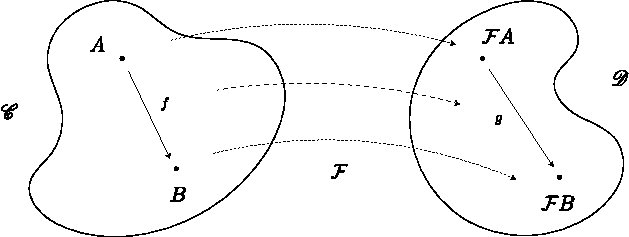
\includegraphics[scale=1]{fig/faith-full.pdf}
	\caption{For all $A, B$, and $g$, a faithful functor sends at \textit{most} one solid arrow in $\cat{C}$ to $g$. A full functor sends at \textit{least} one solid arrow in $\cat{C}$ to $g$.}
\end{figure}

\begin{ex}
The inclusion functor from $\cat{S}$ to $\cat{C}$ is always faithful, and it's full if and only if $\cat{S}$ is a full subcategory.
\end{ex}

%%%%%%%%%%%%%%%%%%%%
% Natural Transformations
%%%%%%%%%%%%%%%%%%%%

\section{Natural Transformations}

When functors have the same domain and codomain, we can define a map between them.

\begin{defn}
Suppose $\mathcal{F},\mathcal{G}:\cat{A}\to \cat{B}$ are functors. Then a \textbf{natural transformation} $\alpha:\mathcal{F}\to \mathcal{G}$ is a family
\[
	(\alpha_A: \mathcal{F}A \to \mathcal{G}A)_{A \in \cat{A}}
\] such that the following diagram commutes.
\begin{figure}[H]
	\centering
\begin{tikzcd}
\mathcal{F}A \arrow[d, "\alpha_A"'] \arrow[r, "\mathcal{F}(f)"] & \mathcal{F}A' \arrow[d, "\alpha_{A'}"] \\
\mathcal{G}A \arrow[r, "\mathcal{G}(f)"']                       & \mathcal{G}A'
\end{tikzcd}
\end{figure}

The maps $\alpha_A$ are the \textbf{components} of $\alpha$.
\end{defn}

The diagram above commuting means $\mathcal{G}(f) \circ \alpha_A = \alpha_{A'} \circ \mathcal{F}(f)$, but it's easier to understand the diagram, so you should remember it by that.

Also, the diagram commuting means that there's only one map from $\mathcal{F}A$ to $\mathcal{G}A'$, namely the diagonal of the diagram (which you can construct by taking the composition of either path).

\begin{figure}[H]
	\centering
	\begin{tikzpicture}
		\node (A) at (-1,0) {$\cat{A}$};
		\node (B) at (1,0) {$\cat{B}$};
		\node at (0,0) {$\Downarrow \alpha$};
		\path[->,font=\scriptsize]
			(A) edge [bend left] node[above] {$\mathcal{F}$} (B)
			edge [bend right] node[below] {$\mathcal{G}$} (B);
	\end{tikzpicture}
	\caption{Because we love overloading notation, we'll denote natural transformations with a $\implies$, as in this diagram.}
\end{figure}

Given two natural transformations $\alpha$ and $\beta$, we can form the composition
\[
	(\beta \circ \alpha)_A = \beta_A \circ \alpha_A.
\] Additionally, we can define the identity natural transformation $1_F$ by
\[
	(1_F)_A = 1_{F(A)}.
\] 

\begin{ex}[Even more category inception]
	We can form a category whose objects are functors from $\cat{A}$ to $\cat{B}$ and whose morphisms are natural transformations. This is called the \textbf{functor category} from $\cat{A}$ to $\cat{B}$, and we denote it by $[\cat{A},\cat{B}]$ or $\cat{B}^{\cat{A}}$.
\end{ex}

	For funsies, we'll break down what's going on in the category functor $[2, \cat{C}]$, where $2$ is the discrete category with 2 objects and $\cat{C}$ is arbitrary, by examining what two functors $\mathcal{F}, \mathcal{G} \in \ob([2, \cat{C}])$ do.

\begin{figure}[H]
	\centering
	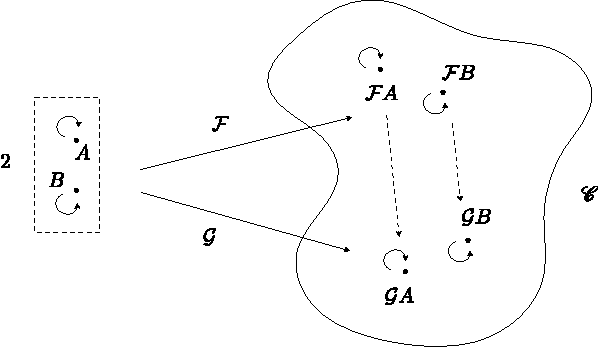
\includegraphics[scale=1]{fig/functor-cat.pdf}
	\caption{Two functors $\mathcal{F}$ and $\mathcal{G}$ in $[2,\cat{C}]$.}
\end{figure}

Although a functor is more than just an object, we can uniquely represent both functors by a pair of objects $(\mathcal{F}A, \mathcal{F}B)$ and $(\mathcal{G}A, \mathcal{G}B)$. A natural transformation between them can then be uniqely represented by a pair of morphisms in $\mathcal{C}$ that run from $\mathcal{F}A\to \mathcal{G}A$ and $\mathcal{F}B\to \mathcal{G}B$ (the dotted lines in the figure). So we've represented $[2, \cat{C}]$ using only 1) pairs objects in $\mathcal{C}$ and 2) pairs of morphisms in $\mathcal{C}$.

Thus structurally, this functor category is the same as $\cat{C} \times \cat{C}$, i.e. $[2, \cat{C}] \cong \cat{C} \times \cat{C}$. This particular case works nicely with the other notation for functor categories, i.e. $\cat{C}^2$.

\begin{defn}
	A \textbf{natural isomorphism} between functors from $\cat{A}$ to $\cat{B}$ is an isomorphism in $[\cat{A},\cat{B}].$
\end{defn}

\begin{prop}
Let $\mathcal{F},\mathcal{G}:\cat{A}\to \cat{B}$ be functors, and let $\alpha:F\implies G$ be a natural transformation between them. Then $\alpha$ is a natural isomorphism if and only if $\alpha_A:\mathcal{F}A\to \mathcal{G}A$ is an isomorphism for all $A \in \cat{A}$.
\end{prop}
\begin{proof}
{\color{red}You should read over your proof again cause it seems a little trivial? This statement kinda is, though?}
\end{proof}

\end{document}
